% this file is called up by the header file
% content in this file will be fed into the main document
% ----------------------- paths to graphics ------------------------
\graphicspath{{figures/}}

% ----------------------- contents start here ------------------------

                       
\chapter{Introduction}

In order to get a proper understanding of gigahertz network channel capacities 
(maximum data transfer rate) and ranges, a theoretical channel model will be 
derived subsequently. The channel model is further supposed highlight signal attenuations 
in various environments, with various factors affecting signal power. \\
The report starts with estabilishing a basic channel in chapter \ref{chap:model}, 
introduces free-space signal losses and specific signal attenuators such as foliage and rainfall.
The resulting channel model is plotted for a given rural scenario in \ref{chap:simulation} 
and channel capacities for a rural highway scenario discussed.\\
An outlook to further improvements to the model is given in chapter \ref{chap:conclusion_outlook}.\\
Furthermore, the channel model discussed in this report is implemented in the accompanying 
python script. Plots generated in chapter \ref{chap:simulation} can be generated for any 
given combination of channel parameters. 




\begin{figure}[htb]
    \centering
    \begin{minipage}{.4\textwidth}
        \centering
        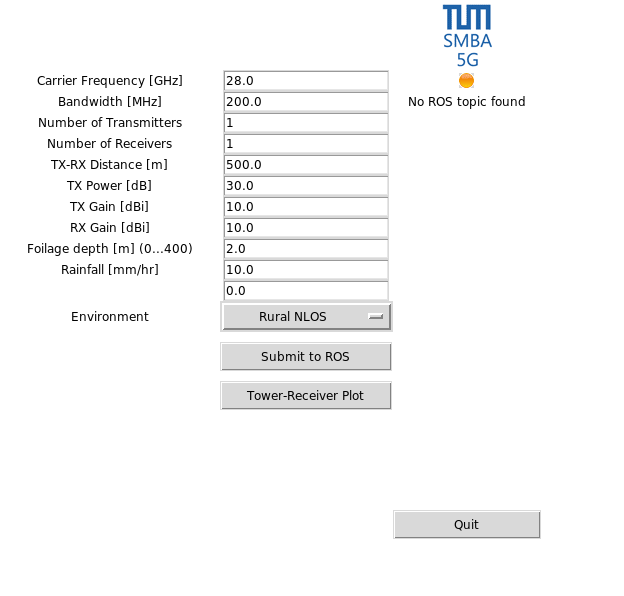
\includegraphics[width=\linewidth]{smba_gui.png}
    \end{minipage}
    \hspace{.1\textwidth}
    \begin{minipage}{.4\textwidth}
        \centering
        %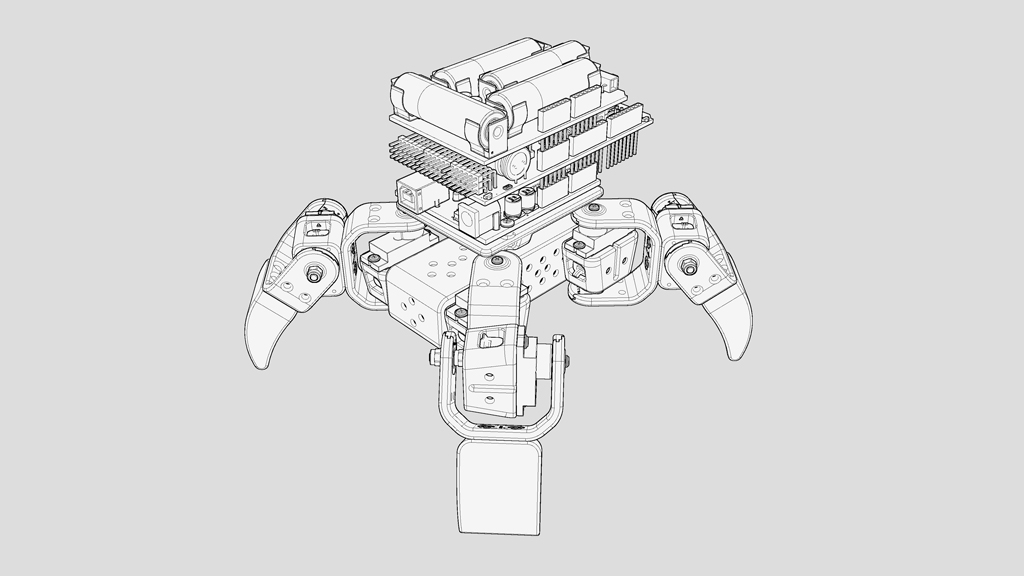
\includegraphics[width=\linewidth]{ALLBOT_isometric_2.jpg}
        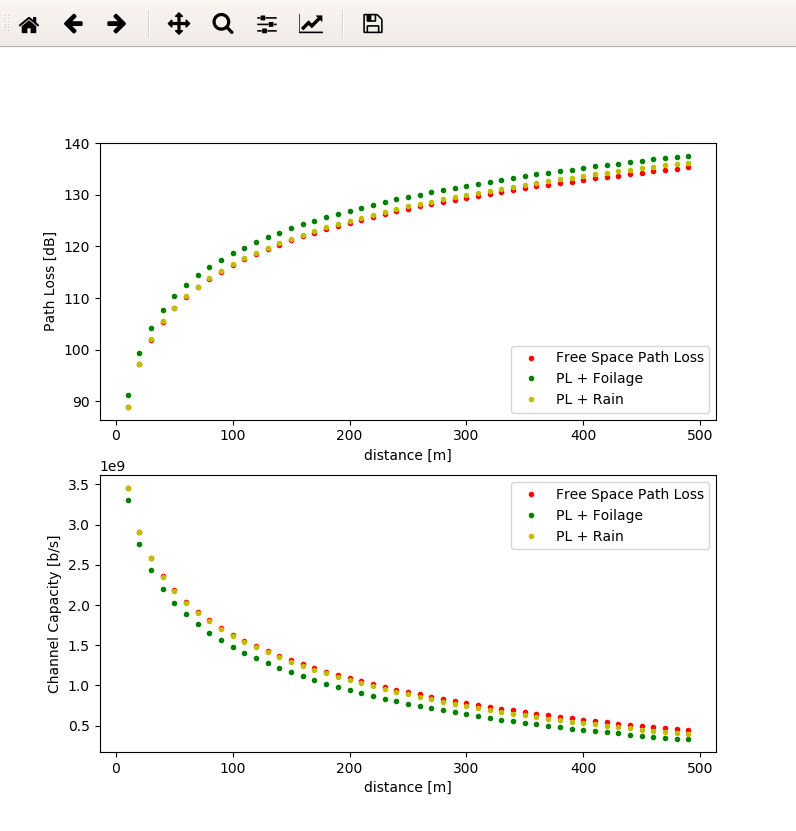
\includegraphics[width=\linewidth]{smba_gui_2.png}
    \end{minipage}
        \caption{Python script GUI to simulate gigahertz channel models and generate path loss and channel
        capacity plots over distance.}
        \label{fig:gui}
\end{figure}


